% ============================================================
%   main.tex —— 深圳大学实验报告（主文件）
% ============================================================

\documentclass[12pt, a4paper]{article}
\usepackage{szu_lab}

\begin{document}

% ============================================================
%   第一页：封面
% ============================================================
\newgeometry{top=3cm, bottom=3cm, left=3.5cm, right=2.5cm}

\begin{center}
    \vspace*{0.5cm}
    {\fontsize{26pt}{30pt}\selectfont\bfseries 深\enspace 圳\enspace 大\enspace 学\enspace 实\enspace 验\enspace 报\enspace 告}
    \vspace{2cm}
\end{center}

\newcommand{\mline}[2]{%
    \noindent\mbox{\zihao{4}\bfseries #1：\underline{\makebox[10cm][l]{#2}}}\\[3ex]%
}

\vspace{0.5cm}
\begin{flushleft}
    \mline{课程名称}{人工智能}
    \mline{实验项目名称}{基于 YOLOv11 的垃圾图像分类}
    \mline{学\hspace{2em}院}{电子与信息工程学院}
    \mline{专\hspace{2em}业}{电子与信息工程}
    \mline{指导教师}{戴林蕙}
    \noindent\mbox{\zihao{4}\bfseries
        报告人：\underline{\makebox[3cm][l]{戴西西(cat)}}%
        \hspace{1.5em}学号：\underline{\makebox[3.5cm][l]{20240615}}%
        \hspace{1.5em}班级：\underline{\makebox[3cm][l]{电信2401}}%
    }\\[3ex]
    \mline{实验时间}{2026 年 4 月 28 日}
    \mline{实验报告提交时间}{2026 年 5 月 18 日}
\end{flushleft}

\vfill
\begin{center}
    {\large \textbf{教\enspace 务\enspace 部\enspace 制}}
\end{center}

\newpage
\restoregeometry


% ============================================================
%   一、实验目的与要求
% ============================================================
\begin{labbox}{一、实验目的与要求：}{}

\begin{itemize}[leftmargin=2em, itemsep=0.3em]
    \item 了解 YOLO 系列算法的发展历程，掌握 YOLOv11 图像分类模型（\texttt{yolo11n-cls}）的网络结构与核心改进。
    \item 学习在 Anaconda 中创建独立虚拟环境，完成 Ultralytics 框架的安装与配置。
    \item 掌握使用公开垃圾分类数据集（\texttt{garbage-classification}，含 6 类）进行数据准备的方法。
    \item 能够在 CPU/GPU 环境下对 YOLOv11n-cls 进行微调训练，理解训练流程与超参数含义。
    \item 学会使用训练好的权重对图片进行推理，解读分类结果与评估指标（Top-1/Top-5 准确率）。
\end{itemize}

\end{labbox}


% ============================================================
%   二、实验方法与步骤
% ============================================================
\begin{labbox}{二、实验方法与步骤：}{}

\begin{enumerate}[leftmargin=2em, itemsep=0.5em]

    \item \textbf{创建并激活虚拟环境}

    打开 Anaconda Prompt，依次执行：
\begin{lstlisting}
conda create -n yolo11 python=3.10 -y
conda activate yolo11
\end{lstlisting}

    \item \textbf{安装 Ultralytics 及依赖}
\begin{lstlisting}
pip install ultralytics torch torchvision pillow matplotlib
\end{lstlisting}

    安装完成后验证：
\begin{lstlisting}
python -c "from ultralytics import YOLO; print('安装成功')"
\end{lstlisting}

    \item \textbf{准备垃圾分类数据集}

    本实验使用 \texttt{garbage-classification} 公开数据集，包含以下 6 个类别，共约 2500 张图片：
    \textbf{cardboard}（纸板）、\textbf{glass}（玻璃）、\textbf{metal}（金属）、
    \textbf{paper}（纸张）、\textbf{plastic}（塑料）、\textbf{trash}（其他垃圾）。
    将数据集解压后放置于项目根目录，目录结构如下：
\begin{lstlisting}
garbage-classification/
  cardboard/   # 纸板类（约 403 张）
  glass/       # 玻璃类（约 501 张）
  metal/       # 金属类（约 410 张）
  paper/       # 纸张类（约 594 张）
  plastic/     # 塑料类（约 482 张）
  trash/       # 其他垃圾（约 137 张）
\end{lstlisting}

    \item \textbf{编写并运行训练脚本}

    新建 \texttt{train.py}，内容见第三节，然后运行：
\begin{lstlisting}
python train.py
\end{lstlisting}

    训练完成后，最佳权重保存于 \texttt{runs/classify/garbage\_exp/weights/best.pt}。

    \item \textbf{推理验证}

    训练完成后运行推理脚本，对 \texttt{test/} 目录中的图片进行分类预测：
\begin{lstlisting}
python predict.py
\end{lstlisting}

    预测结果图片（含 Top-5 置信度柱状图）保存于项目根目录。

\end{enumerate}

\end{labbox}


% ============================================================
%   三、实验过程及内容
% ============================================================
\begin{labbox}{三、实验过程及内容：}{}

\textbf{（1）训练脚本 \texttt{train.py}}

\begin{lstlisting}
from ultralytics import YOLO
import torch

device = 'cuda' if torch.cuda.is_available() else 'cpu'
print(f"使用设备: {device}")

model = YOLO('yolo11n-cls.pt')

results = model.train(
    data='garbage-classification',
    epochs=10,
    imgsz=128,
    batch=16,
    device=device,
    project='runs/classify',
    name='garbage_exp',
    patience=50,
    save=True,
    plots=True
)
print(f"最佳模型: runs/classify/garbage_exp/weights/best.pt")
\end{lstlisting}

\textbf{（2）推理脚本 \texttt{predict.py}}

\begin{lstlisting}
from ultralytics import YOLO
from PIL import Image
import matplotlib.pyplot as plt
import matplotlib
matplotlib.rcParams['font.sans-serif'] = ['SimHei']

model = YOLO('runs/classify/runs/classify/garbage_exp/weights/best.pt')

img_path = 'test/test.jpg'
results = model.predict(img_path, device='cpu')
result = results[0]
top1_class = result.names[result.probs.top1]
top1_conf = result.probs.top1conf.item()
print(f"预测类别: {top1_class}, 置信度: {top1_conf:.2%}")

img = Image.open(img_path)
plt.figure(figsize=(6, 6))
plt.imshow(img)
plt.axis('off')
plt.title(f"预测类别: {top1_class}\n置信度: {top1_conf:.2%}", fontsize=14)
plt.tight_layout()
plt.savefig('result.jpg')
\end{lstlisting}

\textbf{（3）YOLOv11 分类模型核心改进简介}

与 YOLOv8 相比，YOLOv11 主要改进如下：
\begin{itemize}[leftmargin=2em, itemsep=0.2em]
    \item \textbf{C3k2 模块}：改进跨阶段部分网络，在保持精度的前提下减少约 22\% 参数量，更适合轻量级推理。
    \item \textbf{C2PSA 注意力机制}：在颈部引入位置敏感注意力，增强对细粒度特征的提取能力。
    \item \textbf{统一任务接口}：检测、分类、分割共用同一套训练代码，切换任务只需更换模型文件。
\end{itemize}

\textbf{（4）测试图片推理结果}

对 \texttt{test/} 目录中的 4 张图片进行推理，结果如下：

\begin{center}
    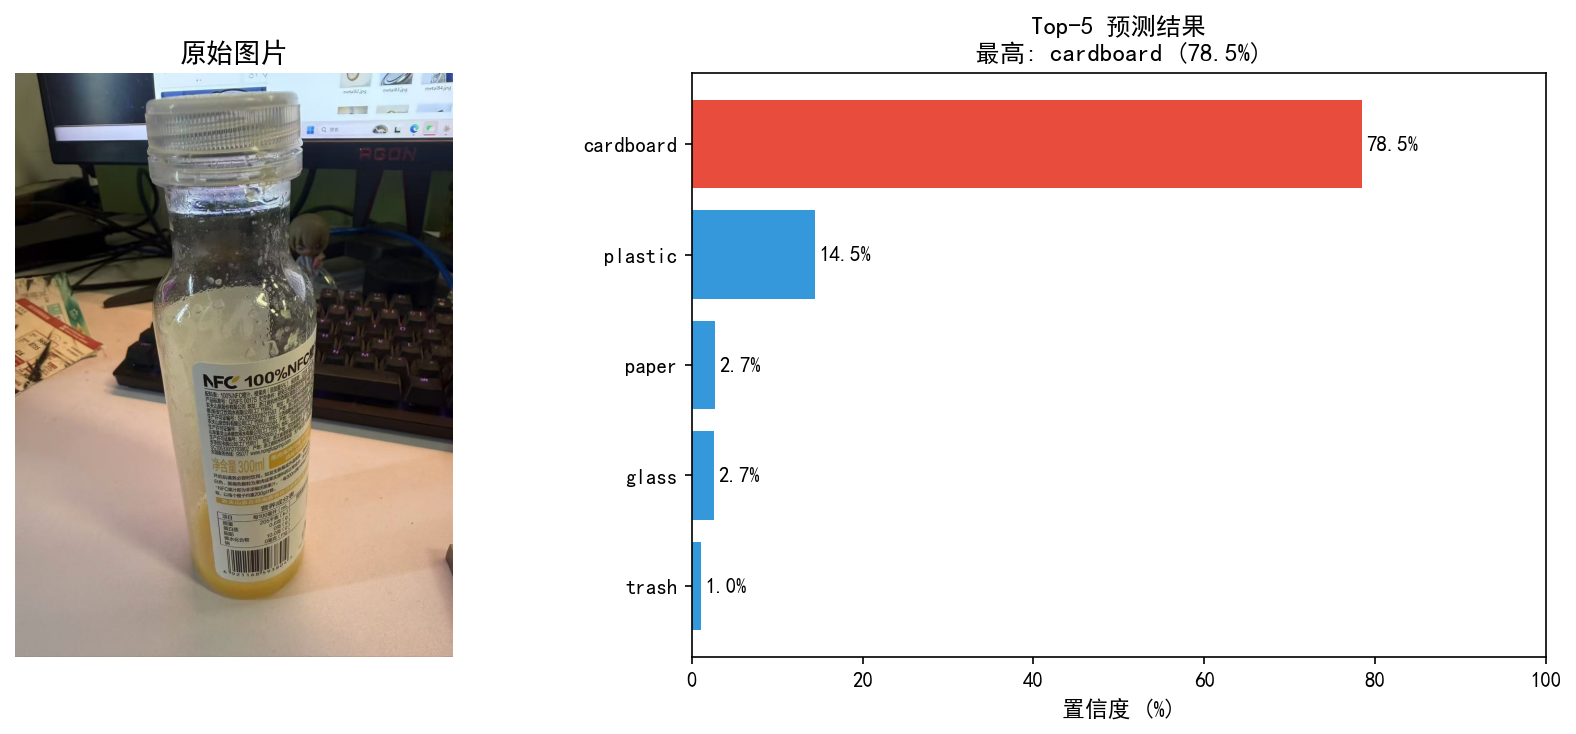
\includegraphics[width=0.88\linewidth]{result_1.png}
    \par\vspace{0.2em}
    {\small 图1\quad 测试图片1推理结果（预测类别：cardboard，置信度 78.46\%）}
\end{center}

\begin{center}
    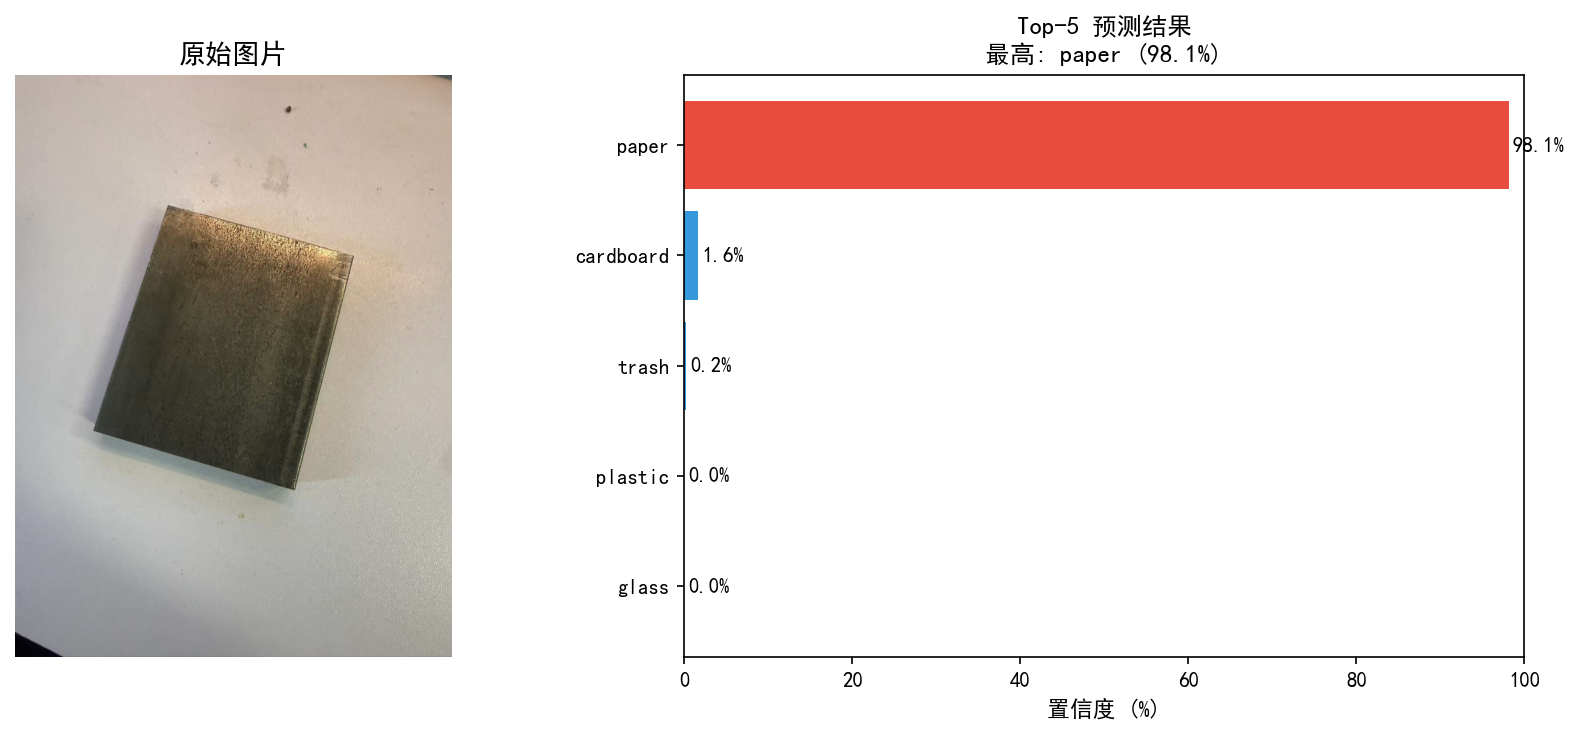
\includegraphics[width=0.88\linewidth]{result_2.png}
    \par\vspace{0.2em}
    {\small 图2\quad 测试图片2推理结果（预测类别：paper，置信度 98.12\%）}
\end{center}

\begin{center}
    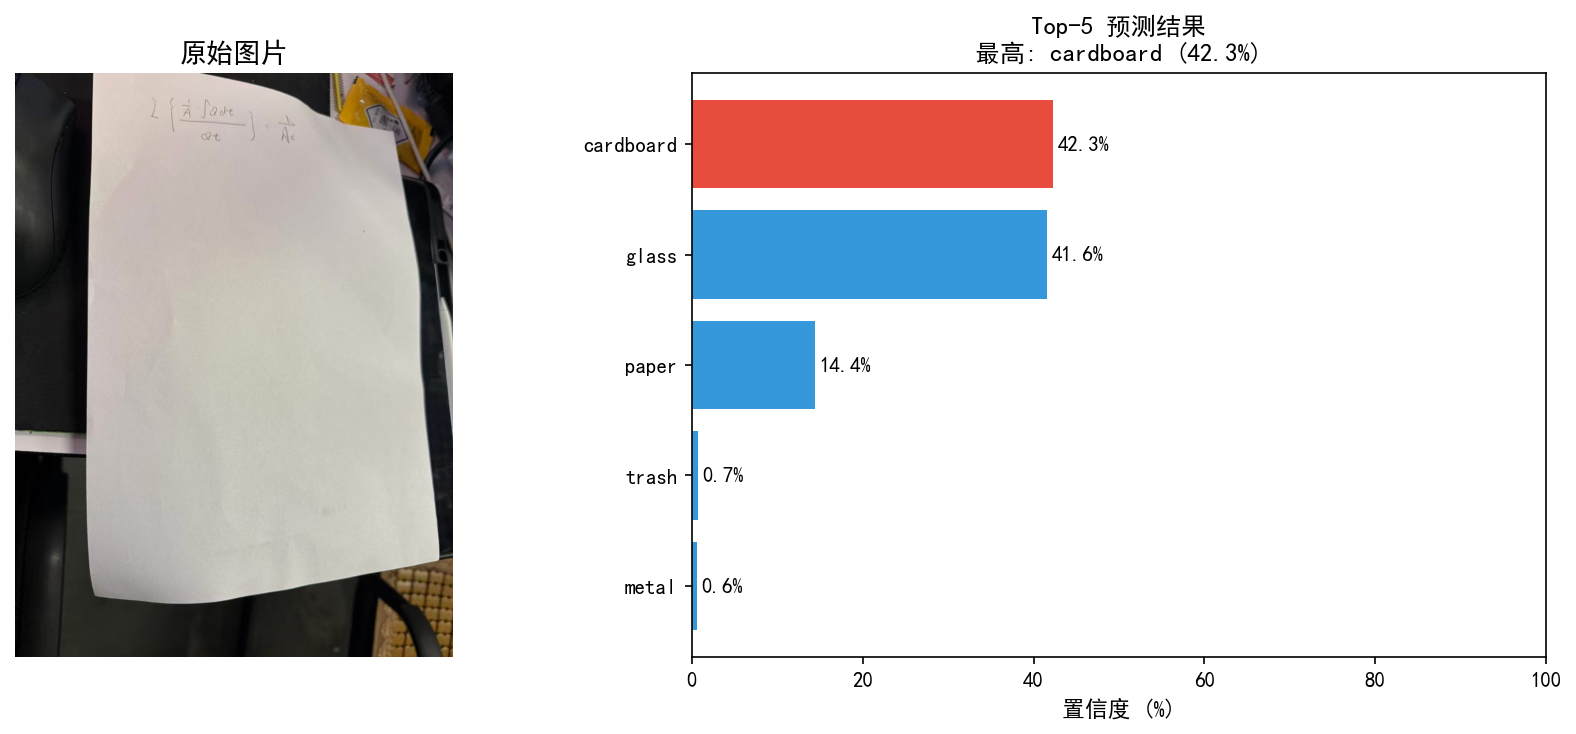
\includegraphics[width=0.88\linewidth]{result_3.png}
    \par\vspace{0.2em}
    {\small 图3\quad 测试图片3推理结果（预测类别：cardboard，置信度 42.31\%）}
\end{center}

\begin{center}
    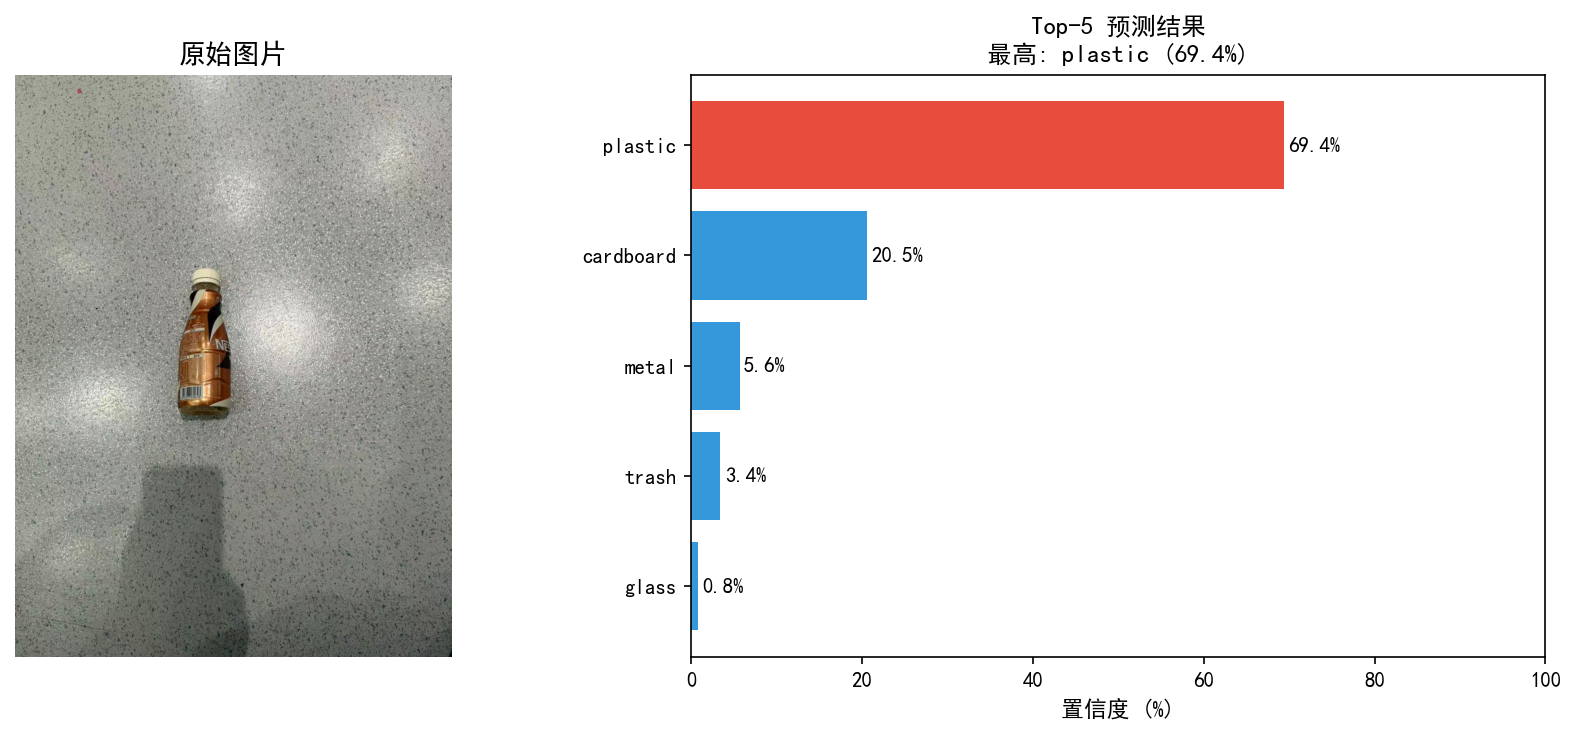
\includegraphics[width=0.88\linewidth]{result_4.png}
    \par\vspace{0.2em}
    {\small 图4\quad 测试图片4推理结果（预测类别：plastic，置信度 69.42\%）}
\end{center}

\end{labbox}


% ============================================================
%   四、数据处理与分析
% ============================================================
\begin{labbox}{四、数据处理与分析：}{}

以实际训练 10 个 epoch 的结果为例（数据来自 \texttt{results.csv}）：

\vspace{0.3cm}
\begin{center}
\begin{tabular}{|c|c|c|c|}
    \hline
    \textbf{Epoch} & \textbf{train/loss} & \textbf{Top-1 准确率} & \textbf{Top-5 准确率} \\
    \hline
    1  & 1.378 & 72.44\% & 99.02\% \\
    2  & 0.806 & 80.31\% & 99.80\% \\
    4  & 0.622 & 81.30\% & 99.61\% \\
    6  & 0.485 & 87.99\% & 99.61\% \\
    8  & 0.373 & 83.86\% & 99.80\% \\
    10 & 0.301 & 88.19\% & 100.00\% \\
    \hline
\end{tabular}
\end{center}
\vspace{0.3cm}

\textbf{各指标含义：}
\begin{itemize}[leftmargin=2em, itemsep=0.2em]
    \item \textbf{train/loss}：训练集交叉熵损失，越低说明模型对训练样本的拟合越好。
    \item \textbf{Top-1 准确率}：预测概率最高的类别与真实类别一致的比例，是分类任务最核心的指标。
    \item \textbf{Top-5 准确率}：真实类别出现在预测概率前 5 名中的比例，反映模型的候选召回能力。
\end{itemize}

\vspace{0.3cm}
\textbf{训练曲线与混淆矩阵：}

\begin{center}
    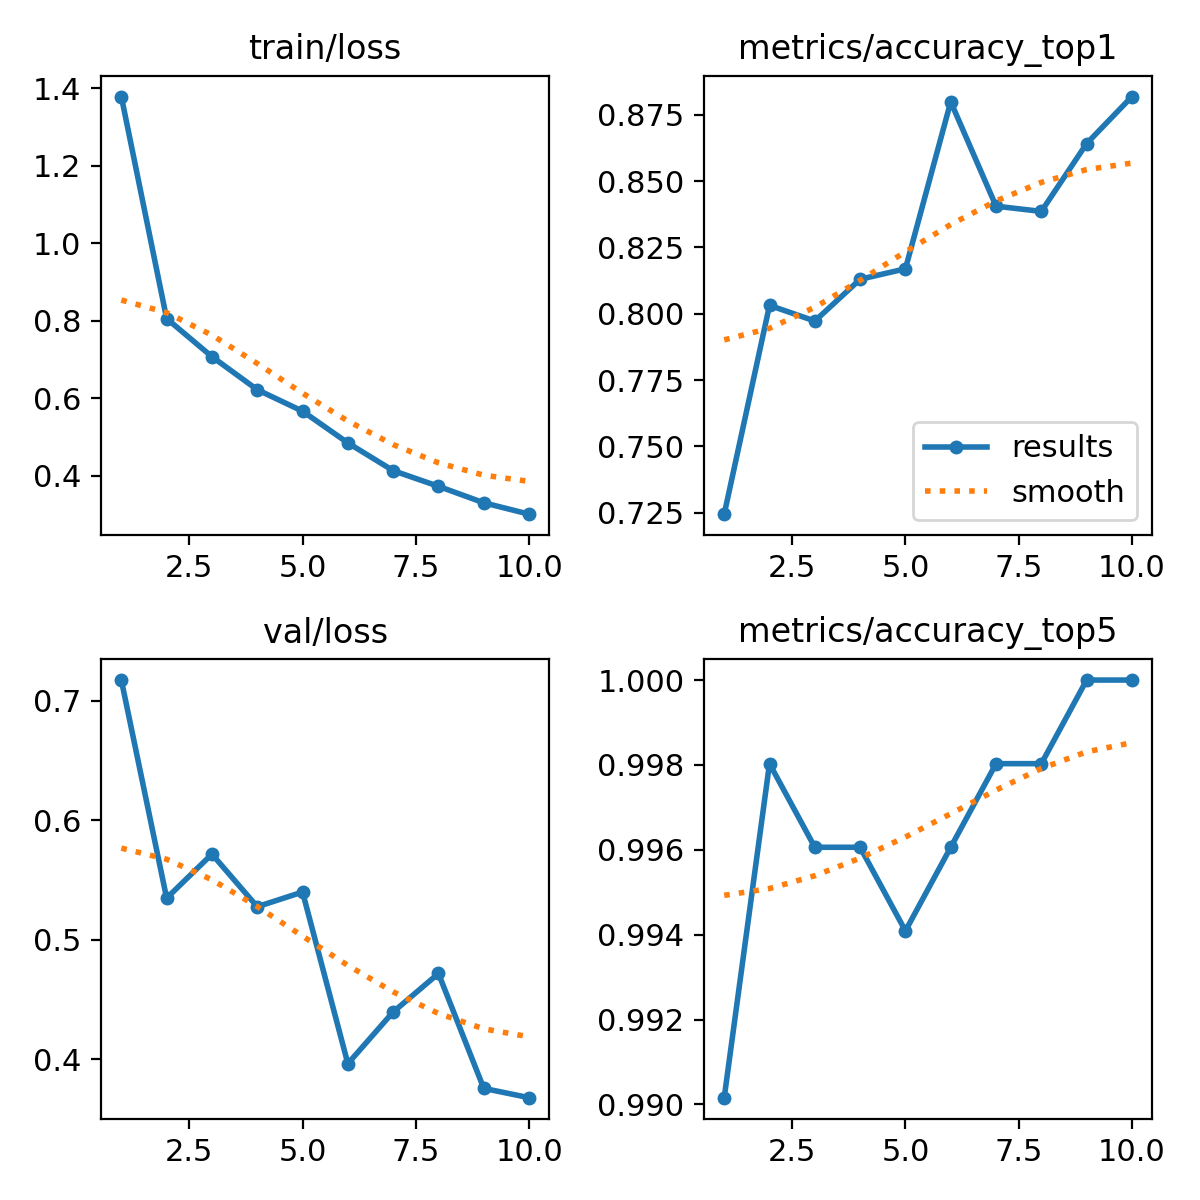
\includegraphics[width=0.88\linewidth]{train_results.png}
    \par\vspace{0.2em}
    {\small 图5\quad 训练过程损失与准确率曲线（10 个 epoch）}
\end{center}

\begin{center}
    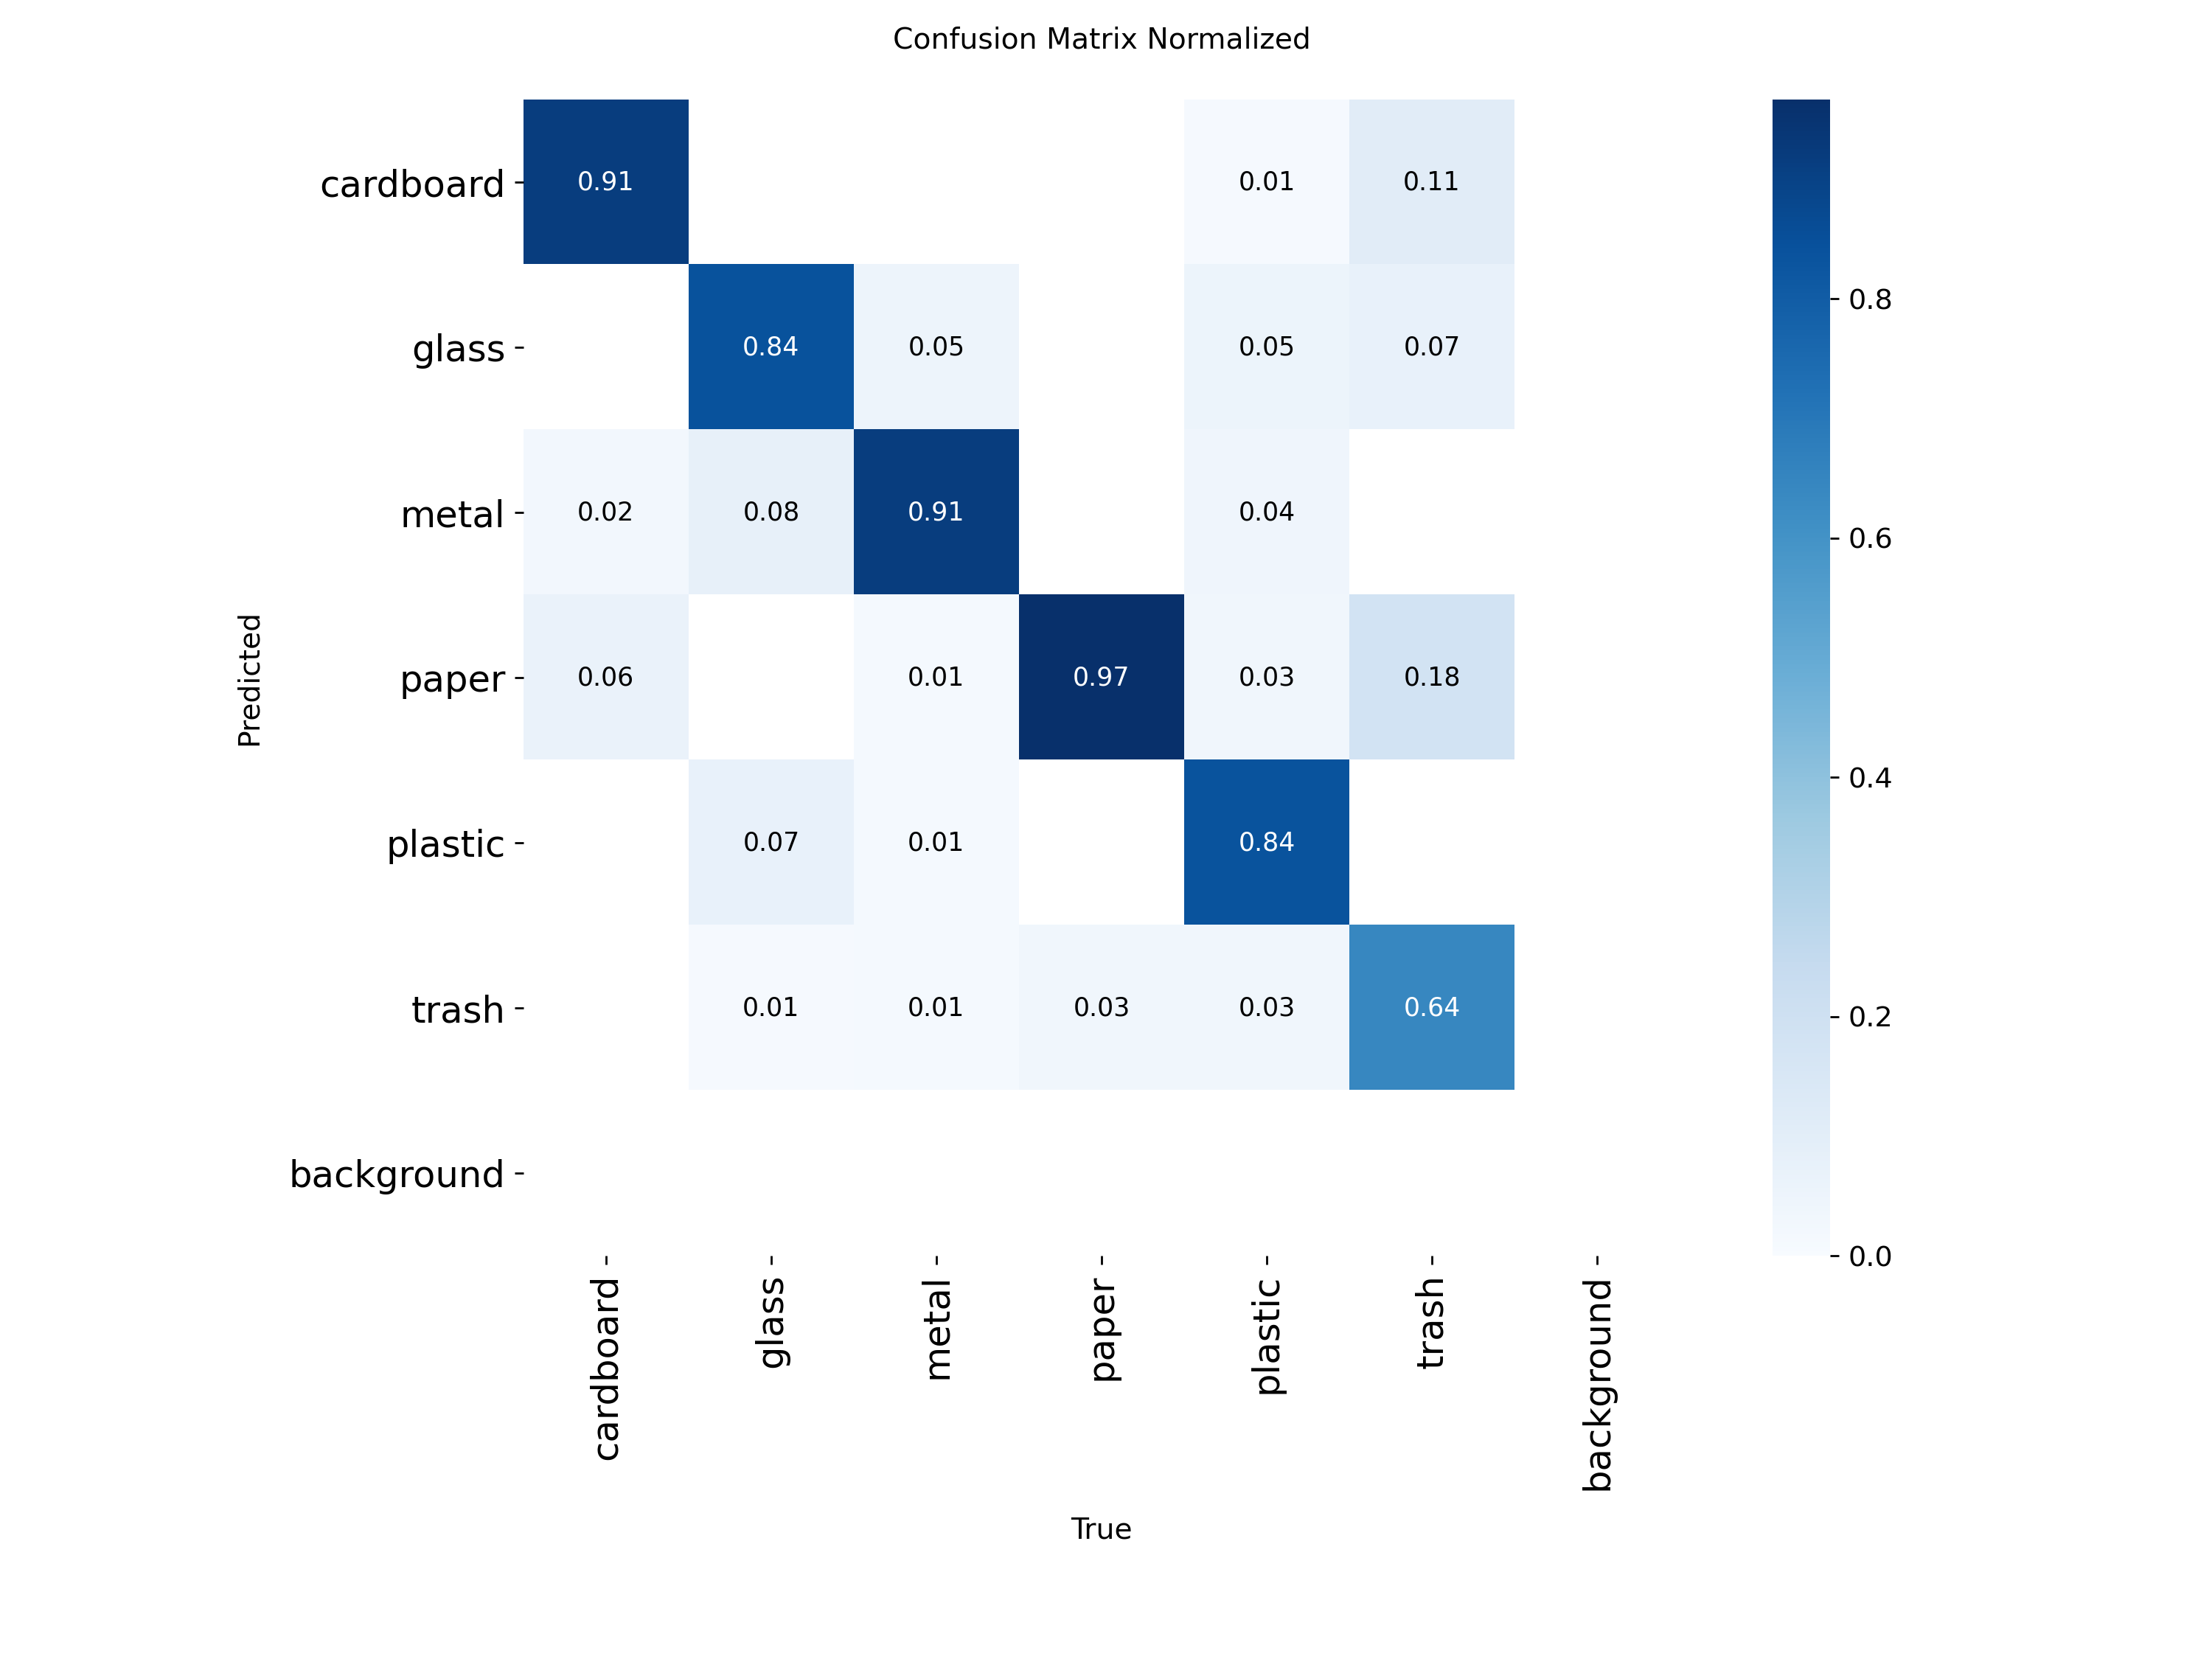
\includegraphics[width=0.72\linewidth]{confusion_matrix.png}
    \par\vspace{0.2em}
    {\small 图6\quad 归一化混淆矩阵（验证集）}
\end{center}

\vspace{0.2cm}
由训练曲线可见，损失在前 6 个 epoch 快速下降，Top-1 准确率从 72.4\% 提升至 88.2\%，
Top-5 准确率在第 9 个 epoch 即达到 100\%，说明模型对 6 类垃圾的区分能力良好。
混淆矩阵显示 paper 与 cardboard 之间存在少量混淆，这与两类材质外观相近有关，
可通过增加训练数据或数据增强进一步改善。

\end{labbox}


% ============================================================
%   五、实验结论
% ============================================================
\newpage
\begin{labbox}{五、实验结论：}{}

\begin{enumerate}[leftmargin=2em, itemsep=0.4em]
    \item 本实验基于 YOLOv11n-cls 预训练权重，在 \texttt{garbage-classification} 数据集上完成了
          垃圾图像六分类任务的完整训练与推理流程，验证了 Ultralytics 框架对分类任务的良好支持。

    \item 训练仅用 10 个 epoch，最终验证集 Top-1 准确率达到 \textbf{88.19\%}，
          Top-5 准确率达到 \textbf{100\%}，说明 YOLOv11n-cls 在小规模数据集上具有较强的迁移学习能力。

    \item 推理结果表明，模型对 paper（98.12\%）、plastic（69.42\%）等类别置信度较高；
          cardboard 与 glass 之间存在一定混淆（图3置信度差距较小），
          与两类材质在外观上的相似性有关。

    \item 实验中将 \texttt{imgsz} 设为 128、\texttt{batch} 设为 16，
          在 CPU 环境下单 epoch 训练时间约 30 秒，10 个 epoch 共约 5 分钟，
          说明合理调整超参数可显著降低低配环境的训练成本。

    \item 若需进一步提升精度，可采取以下措施：增加训练 epoch 数量；
          使用更大模型（\texttt{yolo11s-cls.pt}）；对 cardboard/glass 类别补充更多样本；
          或在 GPU 环境下以更大 \texttt{imgsz}（如 224）训练。
\end{enumerate}

\end{labbox}

% ---------- 教师评阅区 ----------
\begin{labbox}{}{9cm}
    \hspace{1em}\zihao{-4}指导教师批阅意见：\\[3.5cm]
    \hspace{1em}成绩评定：\\[2cm]
    \hfill 指导教师签字：\hspace{4em} \\
    \hfill \makebox[3em]{}年\makebox[2em]{}月\makebox[2em]{}日\hspace{2em} \\[0.5em]
\end{labbox}

% ---------- 备注 ----------
\begin{labbox}{备注：}{}
    无
\end{labbox}

% ---------- 底部注释 ----------
\begin{spacing}{1.2}
    \zihao{5}
    \noindent 注：\begin{minipage}[t]{0.88\textwidth}
        1、报告内的项目或内容设置，可根据实际情况加以调整和补充。\\
        2、教师批改学生实验报告时间应在学生提交实验报告时间后 10 日内。
    \end{minipage}
\end{spacing}

\end{document}
